\documentclass[../AP_Physics_C.tex]{subfiles}

\begin{document}
	\section{Rotation}
		A \textbf{rigid body} rotates as a unit. \\
		The axis about which an object rotates is the \textbf{axis of rotation}. The \textbf{angular position} $\pmb{\theta}$ of this line is taken relative to a fixed direction, the \textbf{zero angular position}. \\
		\callout{17}{Although its can be changed (if specified), positive angles are conventionally \textbf{counterclockwise} from the zero angular position.}
		Angular dimension is measured using \textbf{radians} (\textbf{rad}), which are dimensionless.
		\[\theta = \frac{s}{r}\]
		A \textbf{revolution} is equal to $360^\circ$, which is also equal to $2\pi\,\rad$.
	\section{Rolling, Torque, and Angular Momentum}
		For an object to \textbf{roll} is for it to move rotationally and translationally along a surface. For an object to roll \textbf{smoothly} is for it not to leave the ground while it is rolling. \\
		\callout{17}{Smooth rolling can be thought of as pure rotation and pure translation or as rotation about a moving contact point.}
		The center of mass of a rolling object moves parallel to the surface. The rest of the object rotates about the center of mass. \\
		The \textbf{arc distance} $\pmb{S}$, the distance covered on the surface, and the velocity about the center of mass are defined as linear variables:
		\begin{align*}
			S &= \theta r & \com{v} &= \omega r
		\end{align*}
		As rolling objects move both translationally and rotationally, they have both translational and rotational kinetic energy.\footnote{
			The parallel axis theorem can be used to calculate the kinetic energy about the contact point.
			\[
				K = \frac{1}{2}I_P\omega^2 = \frac{1}{2}(I_{\com} + Mr^2)\omega^2 = \frac{1}{2}I_{\com}\omega^2 + \frac{1}{2}Mr^2\left(\frac{v_{\com}}{r}\right)^2 = \frac{1}{2}I_{\com}\omega^2 + \frac{1}{2}Mv_{\com}^2		
			\]
			}
		\[K = \frac{1}{2}I_{\com}\omega^2 + \frac{1}{2}Mv_{com}^2\]
		If no slipping occurs, then energy is conserved (even with friction).
		The acceleration about the center of mass follows the pattern of position and velocity.
		\[a_{\com} = \alpha r\]
		\callout{17}{Acceleration is only dependent on the shape of the object. Its mass and radius are irrelevant.}
		For an object to roll smoothly on a slope, three things are required are required:
		\begin{enumerate}
			\item
				The gravitational force must be vertically down.
			\item
				The normal force must be perpendicular to the slope.
			\item
				The force of friction must point up the slope.
		\end{enumerate}
		\callout{17.45}{The frictional and normal forces are applied to the point of contact rather than the center of mass.}
		A force only results in torque if it does not pass through the contact point. The torque can be calculated as the product of the perpendicular components of the force and the radius.
		\[\tau = r_\bot F = rF_\bot = rF\sin\phi\]
		The second law can then be used.
		\[\net{\tau} = I\alpha = I\left(\frac{a_{\com}}{r}\right)\]
		%TODO FBD for Rolling on Slope
		The acceleration of a body rolling smoothly down a slope can be found as such:
		\[a_{\com, x} = \frac{-g\sin\theta}{I + \frac{\com{I}}{Mr^2}}\]
		\subsection{Torque}
			Torque can be defined as a vector for an individual particle moving along any path relative to a fixed point. It is the cross product of $\vec{r}$ and $\vec{F}$.
			\[
				\vec{\tau} = \vec{r} \times \vec{F} = 
					\begin{bmatrix}
				 		r_x & r_y & r_z \\
					\end{bmatrix} \times 
					\begin{bmatrix}
				 		F_x & F_y & F_z
					\end{bmatrix} =
					\begin{bmatrix}
						r_yF_z - r_zF_y \\
						r_xF_z - r_zF_x \\
						r_xF_z - r_yF_z
					\end{bmatrix}
			\]
			The resultant direction can be determined with the right hand rule, pointing the index and middle fingers of the right hand in the directions of the force and radius such that the thumb will point in the resultant direction of torque. \\
			The angle can also be determined using unit vector notation. The product of two unit vectors is always the third. Its sign is dependent on the the \enquote{order} of the unit vectors.
			\begin{center}
				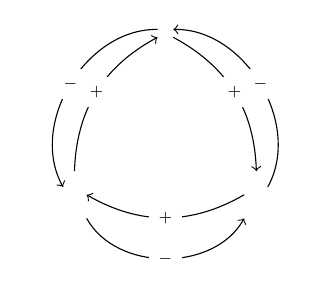
\begin{tikzpicture}
					\node at (0, 2) {\iv};
					\node at (1.155, 0) {\jv};
					\node at (-1.155, 0) {\kv};
					\draw[->] (0.1, 2) to[bend left] node[midway, fill = white]{\tiny$+$} (1.155, 0.3);
					\draw[->] (1, 0) to[bend left] node[midway, fill = white]{\tiny$+$} (-1, 0);
					\draw[->] (-1.155, 0.3) to[bend left] node[midway, fill = white]{\tiny$+$} (-0.1, 2);
					\draw[->] (-0.1, 2.1) to[bend right = 60] node[midway, fill = white]{\tiny$-$} (-1.3, 0.1);
					\draw[->] (-1, -0.3) to[bend right = 61] node[midway, fill = white]{\tiny$-$} (1, -0.3);
					\draw[->] (1.3, 0.1) to[bend right = 60] node[midway, fill = white]{\tiny$-$} (0.1, 2.1);
				\end{tikzpicture}	
			\end{center}
		\subsection{Angular Momentum}
			The \textbf{angular momentum} $\pmb{\ell}$ of a particle is equal to the product of its distance and linear momentum.
			\[\vec{\ell} = \vec{r} \times \vec{p} = m(\vec{r} \times \vec{v})\]
			Angular momentum has units of $\mathrm{kgm^2/s}$ (or Js).
			The magnitude of $\vec{\ell}$ is the product of the perpendicular components of $\vec{r}$ and $\vec{p}$.
			\[\ell = r_\bot p = rp_\bot = rp\sin\phi = mrv\sin\phi\]
			Newton's second law can be rewritten to state that torque is the time derivative of angular momentum, but in order for this to be true, they must be defined about the same point.\footnote{
				Using the formula for angular momentum, the fact that its time derivative is torque can be shown:
				\[\frac{\d}{\d t}\vec{\ell} = \frac{\d}{\d t}m(\vec{r}\times\vec{v}) = m\vec{r}\left(\frac{\d\vec{v}}{\d t}\right) = m\vec{r}\times \vec{a} = \vec{F}_{\net}\times\vec{r} = \vec{\tau}_{\net}\]
			}
			\[\vec{\tau}_{\net} = \frac{\d \vec{\ell}}{\d t}\]
			The time derivative of \textbf{net angular momentum}, denoted $\vec{L}$, is equal to the sum of the net torques of each particle, denoted $\vec{\Tau}$.
			\[\frac{\d\vec{L}}{\d t} = \vec{\Tau}\]
			If the net external torque on a system is zero, then angular momentum is \emph{conserved}. \\
			Linear momentum can be written as the product of inertia and angular velocity.\footnote{It can be shown that linear momentum is the product of inertia and linear momentum by rewriting its formula or by integrating its time derivative.\begin{align*}\ell &= mrv = mr^2\omega = I\omega \\ &= \int \tau\,\d t = \int I\alpha\,\d t = I\omega\end{align*}}
			\[\ell = I\omega\]
\end{document}